\documentclass{standalone}
\usepackage{tikz}
\usetikzlibrary{patterns, positioning}
\usetikzlibrary{shapes.misc}
\usepackage[outline]{contour}
\contourlength{1.5pt} 


\begin{document}
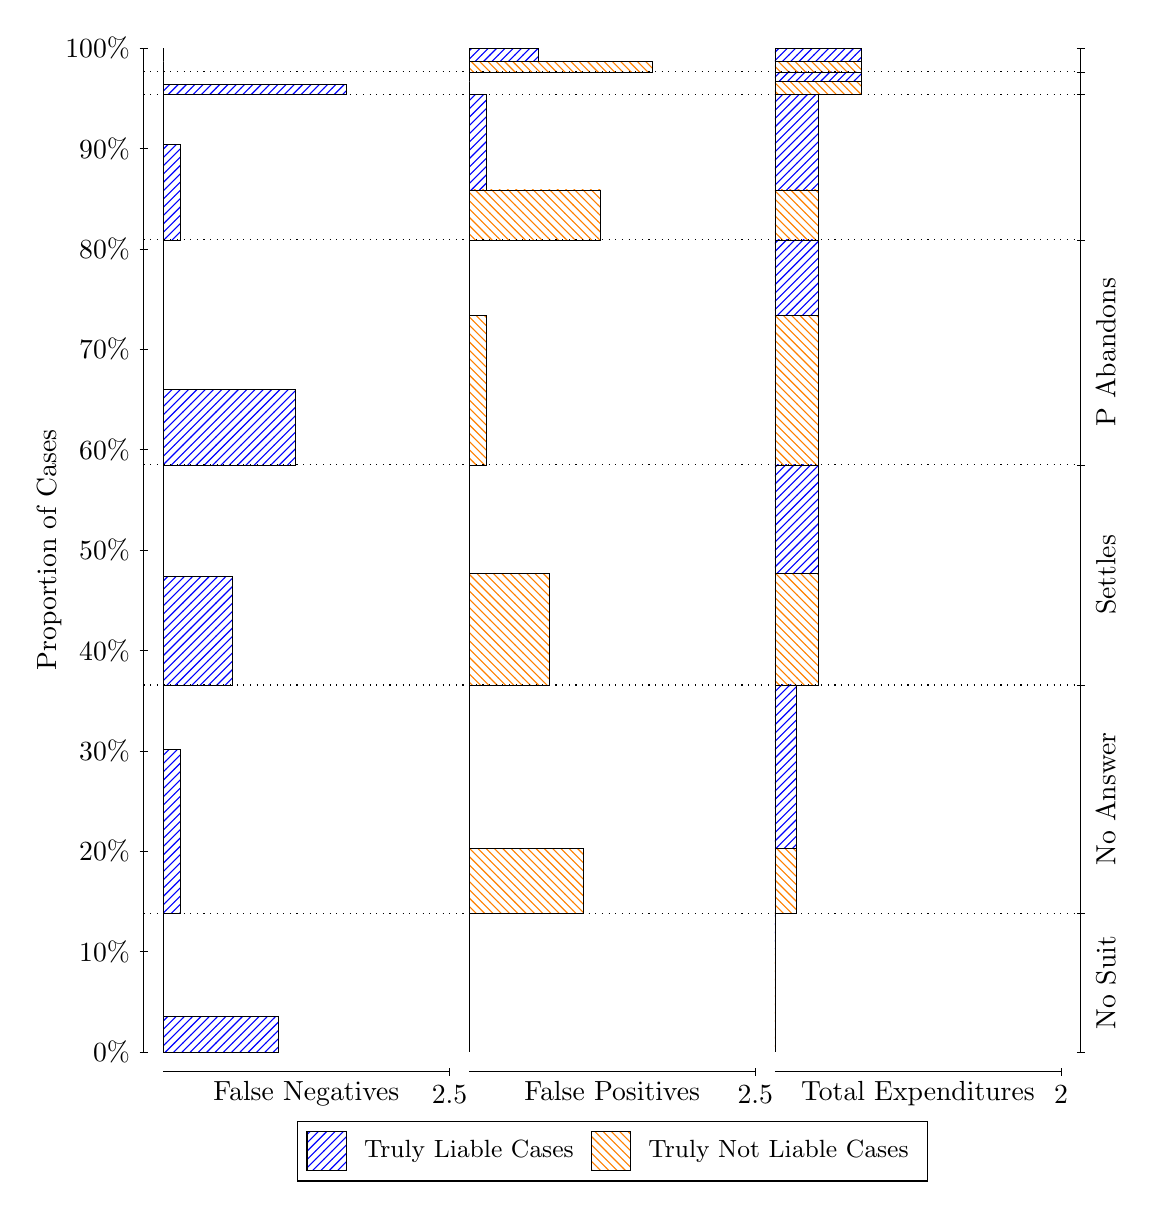
\begin{tikzpicture}
\draw[black, very thin] (1.5,1.75) -- (1.5,14.5);
\node[rotate=90, text=black, anchor=center] at (0.3, 8.125) {Proportion of Cases};
\draw[black, very thin] (1.45,1.75) -- (1.55,1.75);
\node[text=black, anchor=east] at (1.45, 1.75) {0\%};
\draw[black, very thin] (1.45,3.025) -- (1.55,3.025);
\node[text=black, anchor=east] at (1.45, 3.025) {10\%};
\draw[black, very thin] (1.45,4.3) -- (1.55,4.3);
\node[text=black, anchor=east] at (1.45, 4.3) {20\%};
\draw[black, very thin] (1.45,5.575) -- (1.55,5.575);
\node[text=black, anchor=east] at (1.45, 5.575) {30\%};
\draw[black, very thin] (1.45,6.85) -- (1.55,6.85);
\node[text=black, anchor=east] at (1.45, 6.85) {40\%};
\draw[black, very thin] (1.45,8.125) -- (1.55,8.125);
\node[text=black, anchor=east] at (1.45, 8.125) {50\%};
\draw[black, very thin] (1.45,9.4) -- (1.55,9.4);
\node[text=black, anchor=east] at (1.45, 9.4) {60\%};
\draw[black, very thin] (1.45,10.675) -- (1.55,10.675);
\node[text=black, anchor=east] at (1.45, 10.675) {70\%};
\draw[black, very thin] (1.45,11.95) -- (1.55,11.95);
\node[text=black, anchor=east] at (1.45, 11.95) {80\%};
\draw[black, very thin] (1.45,13.225) -- (1.55,13.225);
\node[text=black, anchor=east] at (1.45, 13.225) {90\%};
\draw[black, very thin] (1.45,14.5) -- (1.55,14.5);
\node[text=black, anchor=east] at (1.45, 14.5) {100\%};

\draw[black, very thin] (13.4,1.75) -- (13.4,14.5);
\draw[black, very thin] (13.35,1.75) -- (13.45,1.75);
\node[anchor=west] at (13.35, 1.75) {};
\draw[black, very thin] (13.35,3.5135) -- (13.45,3.5135);
\node[anchor=west] at (13.35, 3.5135) {};
\draw[black, very thin] (13.35,6.4106) -- (13.45,6.4106);
\node[anchor=west] at (13.35, 6.4106) {};
\draw[black, very thin] (13.35,9.2063) -- (13.45,9.2063);
\node[anchor=west] at (13.35, 9.2063) {};
\draw[black, very thin] (13.35,12.063) -- (13.45,12.063);
\node[anchor=west] at (13.35, 12.063) {};
\draw[black, very thin] (13.35,13.908) -- (13.45,13.908);
\node[anchor=west] at (13.35, 13.908) {};
\draw[black, very thin] (13.35,14.198) -- (13.45,14.198);
\node[anchor=west] at (13.35, 14.198) {};
\draw[black, very thin] (13.35,14.5) -- (13.45,14.5);
\node[anchor=west] at (13.35, 14.5) {};

\draw[black, very thin, pattern color=blue, pattern=north east lines] (1.75,1.75) rectangle (3.2033,2.2065);
\draw[black, very thin, pattern color=orange, pattern=north west lines] (1.75,2.2065) rectangle (1.75,3.5135);
\draw[black, very thin, pattern color=blue, pattern=north east lines] (1.75,3.5135) rectangle (1.968,5.5907);
\draw[black, very thin, pattern color=orange, pattern=north west lines] (1.75,5.5907) rectangle (1.75,6.4106);
\draw[black, very thin, pattern color=blue, pattern=north east lines] (1.75,6.4106) rectangle (2.622,7.7881);
\draw[black, very thin, pattern color=orange, pattern=north west lines] (1.75,7.7881) rectangle (1.75,9.2063);
\draw[black, very thin, pattern color=blue, pattern=north east lines] (1.75,9.2063) rectangle (3.4213,10.161);
\draw[black, very thin, pattern color=orange, pattern=north west lines] (1.75,10.161) rectangle (1.75,12.063);
\draw[black, very thin, pattern color=blue, pattern=north east lines] (1.75,12.063) rectangle (1.968,13.273);
\draw[black, very thin, pattern color=orange, pattern=north west lines] (1.75,13.273) rectangle (1.75,13.908);
\draw[black, very thin, pattern color=blue, pattern=north east lines] (1.75,13.908) rectangle (4.0753,14.034);
\draw[black, very thin, pattern color=orange, pattern=north west lines] (1.75,14.034) rectangle (1.75,14.198);
\draw[black, very thin, pattern color=orange, pattern=north west lines] (1.75,14.198) rectangle (1.75,14.326);
\draw[black, very thin, pattern color=blue, pattern=north east lines] (1.75,14.326) rectangle (1.75,14.5);
\draw[black, very thin, pattern color=orange, pattern=north west lines] (5.6333,1.75) rectangle (5.6333,3.057);
\draw[black, very thin, pattern color=blue, pattern=north east lines] (5.6333,3.057) rectangle (5.6333,3.5135);
\draw[black, very thin, pattern color=orange, pattern=north west lines] (5.6333,3.5135) rectangle (7.0867,4.3334);
\draw[black, very thin, pattern color=blue, pattern=north east lines] (5.6333,4.3334) rectangle (5.6333,6.4106);
\draw[black, very thin, pattern color=orange, pattern=north west lines] (5.6333,6.4106) rectangle (6.6507,7.8288);
\draw[black, very thin, pattern color=blue, pattern=north east lines] (5.6333,7.8288) rectangle (5.6333,9.2063);
\draw[black, very thin, pattern color=orange, pattern=north west lines] (5.6333,9.2063) rectangle (5.8513,11.109);
\draw[black, very thin, pattern color=blue, pattern=north east lines] (5.6333,11.109) rectangle (5.6333,12.063);
\draw[black, very thin, pattern color=orange, pattern=north west lines] (5.6333,12.063) rectangle (7.3047,12.698);
\draw[black, very thin, pattern color=blue, pattern=north east lines] (5.6333,12.698) rectangle (5.8513,13.908);
\draw[black, very thin, pattern color=orange, pattern=north west lines] (5.6333,13.908) rectangle (5.6333,14.072);
\draw[black, very thin, pattern color=blue, pattern=north east lines] (5.6333,14.072) rectangle (5.6333,14.198);
\draw[black, very thin, pattern color=orange, pattern=north west lines] (5.6333,14.198) rectangle (7.9587,14.326);
\draw[black, very thin, pattern color=blue, pattern=north east lines] (5.6333,14.326) rectangle (6.5053,14.5);
\draw[black, very thin, pattern color=orange, pattern=north west lines] (9.5167,1.75) rectangle (9.5167,3.057);
\draw[black, very thin, pattern color=blue, pattern=north east lines] (9.5167,3.057) rectangle (9.5167,3.5135);
\draw[black, very thin, pattern color=orange, pattern=north west lines] (9.5167,3.5135) rectangle (9.7892,4.3334);
\draw[black, very thin, pattern color=blue, pattern=north east lines] (9.5167,4.3334) rectangle (9.7892,6.4106);
\draw[black, very thin, pattern color=orange, pattern=north west lines] (9.5167,6.4106) rectangle (10.062,7.8288);
\draw[black, very thin, pattern color=blue, pattern=north east lines] (9.5167,7.8288) rectangle (10.062,9.2063);
\draw[black, very thin, pattern color=orange, pattern=north west lines] (9.5167,9.2063) rectangle (10.062,11.109);
\draw[black, very thin, pattern color=blue, pattern=north east lines] (9.5167,11.109) rectangle (10.062,12.063);
\draw[black, very thin, pattern color=orange, pattern=north west lines] (9.5167,12.063) rectangle (10.062,12.698);
\draw[black, very thin, pattern color=blue, pattern=north east lines] (9.5167,12.698) rectangle (10.062,13.908);
\draw[black, very thin, pattern color=orange, pattern=north west lines] (9.5167,13.908) rectangle (10.607,14.072);
\draw[black, very thin, pattern color=blue, pattern=north east lines] (9.5167,14.072) rectangle (10.607,14.198);
\draw[black, very thin, pattern color=orange, pattern=north west lines] (9.5167,14.198) rectangle (10.607,14.326);
\draw[black, very thin, pattern color=blue, pattern=north east lines] (9.5167,14.326) rectangle (10.607,14.5);
\draw[black, dotted] (1.5,3.5135) -- (13.4,3.5135);
\draw[black, dotted] (1.5,6.4106) -- (13.4,6.4106);
\draw[black, dotted] (1.5,9.2063) -- (13.4,9.2063);
\draw[black, dotted] (1.5,12.063) -- (13.4,12.063);
\draw[black, dotted] (1.5,13.908) -- (13.4,13.908);
\draw[black, dotted] (1.5,14.198) -- (13.4,14.198);
\draw[black, very thin] (1.75,1.5) -- (5.3833,1.5);
\node[text=black, anchor=north] at (3.5667, 1.5) {False Negatives};
\draw[black, very thin] (5.3833,1.45) -- (5.3833,1.55);
\node[text=black, anchor=north] at (5.3833, 1.45) {2.5};

\draw[black, very thin] (5.6333,1.5) -- (9.2667,1.5);
\node[text=black, anchor=north] at (7.45, 1.5) {False Positives};
\draw[black, very thin] (9.2667,1.45) -- (9.2667,1.55);
\node[text=black, anchor=north] at (9.2667, 1.45) {2.5};

\draw[black, very thin] (9.5167,1.5) -- (13.15,1.5);
\node[text=black, anchor=north] at (11.333, 1.5) {Total Expenditures};
\draw[black, very thin] (13.15,1.45) -- (13.15,1.55);
\node[text=black, anchor=north] at (13.15, 1.45) {2};

\node[text=black, centered, rotate=90] at (13.72, 2.6317) {\contour{white}{No Suit}};
\node[text=black, centered, rotate=90] at (13.72, 4.962) {\contour{white}{No Answer}};
\node[text=black, centered, rotate=90] at (13.72, 7.8084) {\contour{white}{Settles}};
\node[text=black, centered, rotate=90] at (13.72, 10.635) {\contour{white}{P Abandons}};




\draw (7.449999999999999,1.5) node[draw=none] (baseCoordinate) {};
\begin{scope}[align=center]
        \matrix[scale=0.5, draw=black, below=0.5cm of baseCoordinate, nodes={draw}, column sep=0.1cm]{
            \node[rectangle, draw, minimum width=0.5cm, minimum height=0.5cm, pattern color=blue, pattern=north east lines] {}; &
            \node[draw=none, font=\small, text=black] (B) {Truly Liable Cases}; &
            \node[rectangle, draw, minimum width=0.5cm, minimum height=0.5cm, pattern color=orange, pattern=north west lines] {}; &
            \node[draw=none, font=\small, text=black] (B) {Truly Not Liable Cases}; \\
            };
\end{scope}

\end{tikzpicture}
\end{document}